\documentclass[1p]{elsarticle_modified}
%\bibliographystyle{elsarticle-num}

%\usepackage[colorlinks]{hyperref}
%\usepackage{abbrmath_seonhwa} %\Abb, \Ascr, \Acal ,\Abf, \Afrak
\usepackage{amsfonts}
\usepackage{amssymb}
\usepackage{amsmath}
\usepackage{amsthm}
\usepackage{scalefnt}
\usepackage{amsbsy}
\usepackage{kotex}
\usepackage{caption}
\usepackage{subfig}
\usepackage{color}
\usepackage{graphicx}
\usepackage{xcolor} %% white, black, red, green, blue, cyan, magenta, yellow
\usepackage{float}
\usepackage{setspace}
\usepackage{hyperref}

\usepackage{tikz}
\usetikzlibrary{arrows}

\usepackage{multirow}
\usepackage{array} % fixed length table
\usepackage{hhline}

%%%%%%%%%%%%%%%%%%%%%
\makeatletter
\renewcommand*\env@matrix[1][\arraystretch]{%
	\edef\arraystretch{#1}%
	\hskip -\arraycolsep
	\let\@ifnextchar\new@ifnextchar
	\array{*\c@MaxMatrixCols c}}
\makeatother %https://tex.stackexchange.com/questions/14071/how-can-i-increase-the-line-spacing-in-a-matrix
%%%%%%%%%%%%%%%

\usepackage[normalem]{ulem}

\newcommand{\msout}[1]{\ifmmode\text{\sout{\ensuremath{#1}}}\else\sout{#1}\fi}
%SOURCE: \msout is \stkout macro in https://tex.stackexchange.com/questions/20609/strikeout-in-math-mode

\newcommand{\cancel}[1]{
	\ifmmode
	{\color{red}\msout{#1}}
	\else
	{\color{red}\sout{#1}}
	\fi
}

\newcommand{\add}[1]{
	{\color{blue}\uwave{#1}}
}

\newcommand{\replace}[2]{
	\ifmmode
	{\color{red}\msout{#1}}{\color{blue}\uwave{#2}}
	\else
	{\color{red}\sout{#1}}{\color{blue}\uwave{#2}}
	\fi
}

\newcommand{\Sol}{\mathcal{S}} %segment
\newcommand{\D}{D} %diagram
\newcommand{\A}{\mathcal{A}} %arc


%%%%%%%%%%%%%%%%%%%%%%%%%%%%%5 test

\def\sl{\operatorname{\textup{SL}}(2,\Cbb)}
\def\psl{\operatorname{\textup{PSL}}(2,\Cbb)}
\def\quan{\mkern 1mu \triangleright \mkern 1mu}

\theoremstyle{definition}
\newtheorem{thm}{Theorem}[section]
\newtheorem{prop}[thm]{Proposition}
\newtheorem{lem}[thm]{Lemma}
\newtheorem{ques}[thm]{Question}
\newtheorem{cor}[thm]{Corollary}
\newtheorem{defn}[thm]{Definition}
\newtheorem{exam}[thm]{Example}
\newtheorem{rmk}[thm]{Remark}
\newtheorem{alg}[thm]{Algorithm}

\newcommand{\I}{\sqrt{-1}}
\begin{document}

%\begin{frontmatter}
%
%\title{Boundary parabolic representations of knots up to 8 crossings}
%
%%% Group authors per affiliation:
%\author{Yunhi Cho} 
%\address{Department of Mathematics, University of Seoul, Seoul, Korea}
%\ead{yhcho@uos.ac.kr}
%
%
%\author{Seonhwa Kim} %\fnref{s_kim}}
%\address{Center for Geometry and Physics, Institute for Basic Science, Pohang, 37673, Korea}
%\ead{ryeona17@ibs.re.kr}
%
%\author{Hyuk Kim}
%\address{Department of Mathematical Sciences, Seoul National University, Seoul 08826, Korea}
%\ead{hyukkim@snu.ac.kr}
%
%\author{Seokbeom Yoon}
%\address{Department of Mathematical Sciences, Seoul National University, Seoul, 08826,  Korea}
%\ead{sbyoon15@snu.ac.kr}
%
%\begin{abstract}
%We find all boundary parabolic representation of knots up to 8 crossings.
%
%\end{abstract}
%\begin{keyword}
%    \MSC[2010] 57M25 
%\end{keyword}
%
%\end{frontmatter}

%\linenumbers
%\tableofcontents
%
\newcommand\colored[1]{\textcolor{white}{\rule[-0.35ex]{0.8em}{1.4ex}}\kern-0.8em\color{red} #1}%
%\newcommand\colored[1]{\textcolor{white}{ #1}\kern-2.17ex	\textcolor{white}{ #1}\kern-1.81ex	\textcolor{white}{ #1}\kern-2.15ex\color{red}#1	}

{\Large $\underline{12a_{0537}~(K12a_{0537})}$}

\setlength{\tabcolsep}{10pt}
\renewcommand{\arraystretch}{1.6}
\vspace{1cm}\begin{tabular}{m{100pt}>{\centering\arraybackslash}m{274pt}}
\multirow{5}{120pt}{
	\centering
	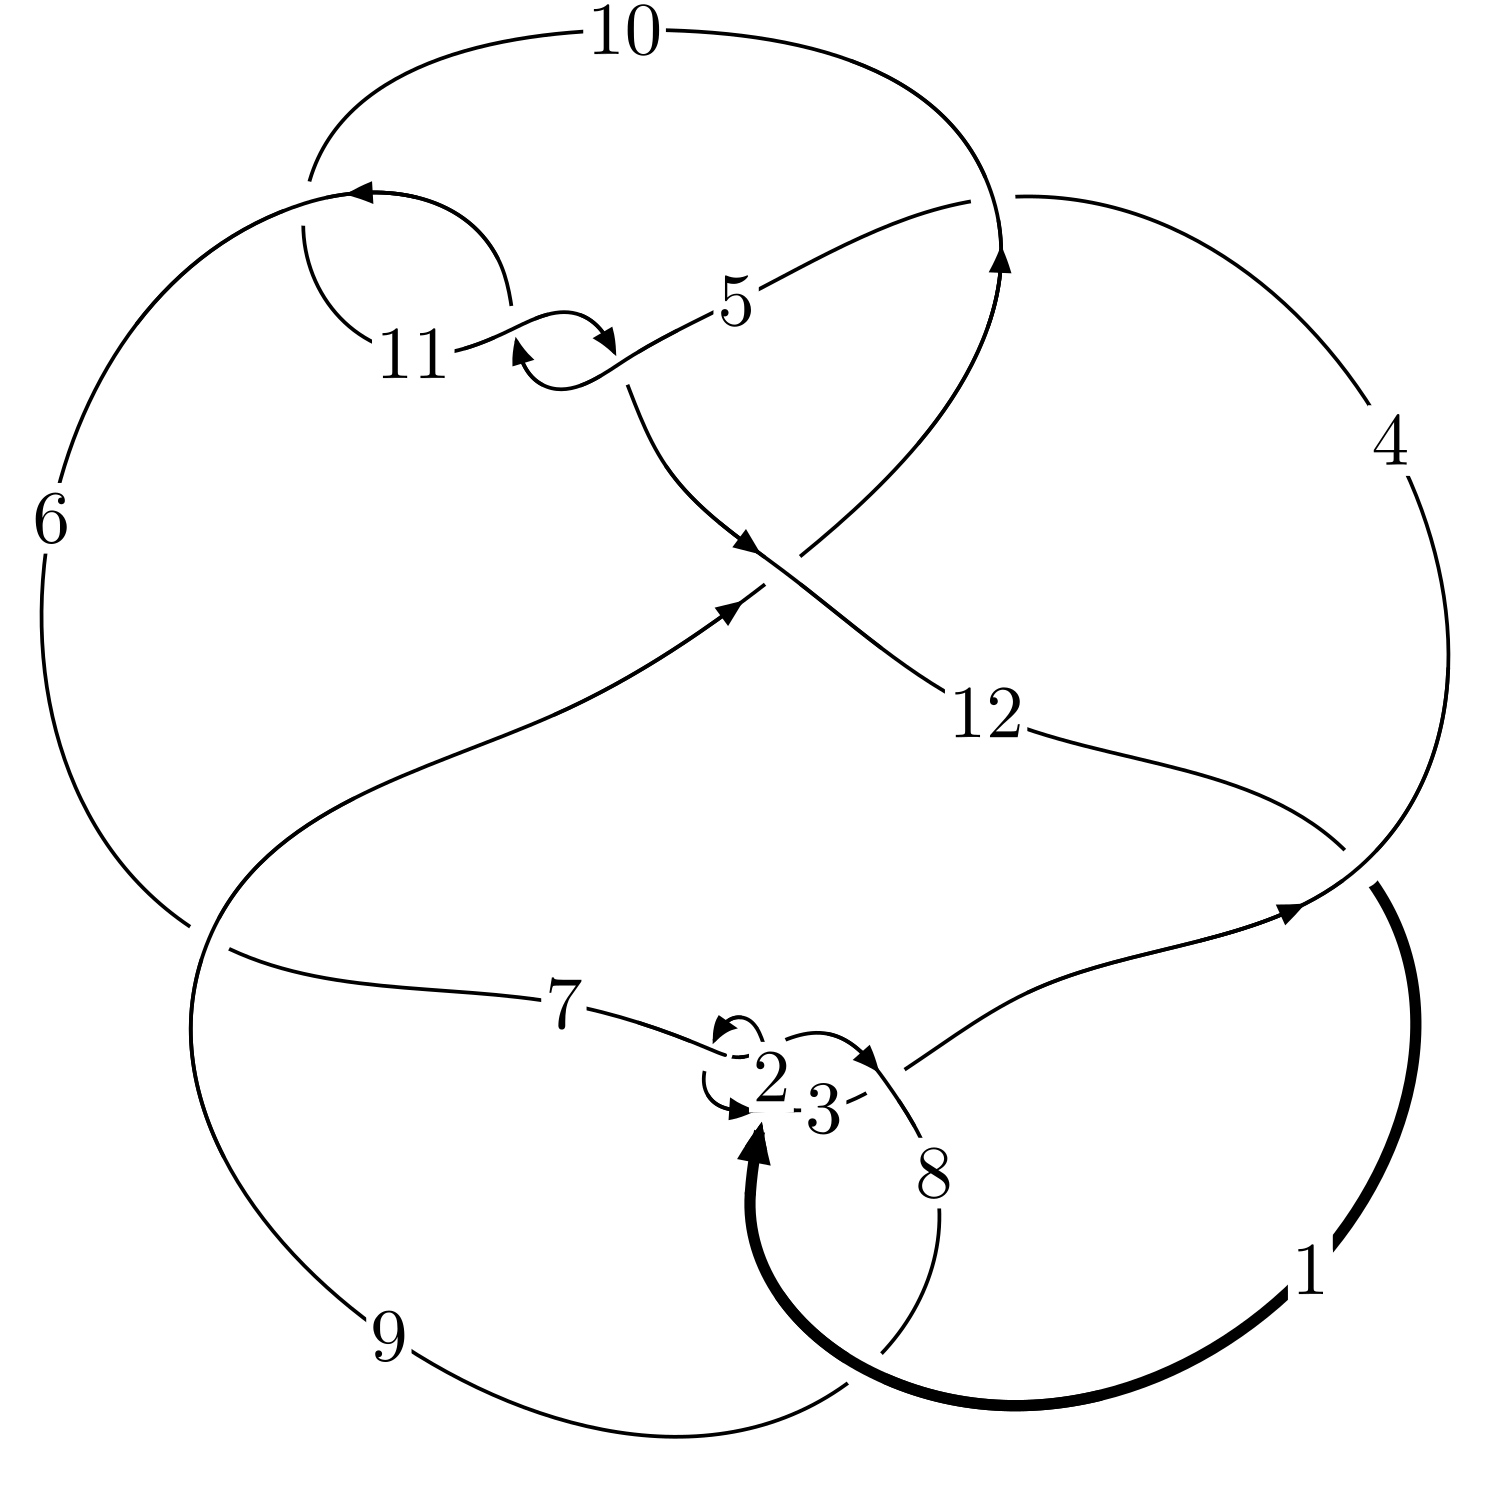
\includegraphics[width=112pt]{../../../GIT/diagram.site/Diagrams/png/1338_12a_0537.png}\\
\ \ \ A knot diagram\footnotemark}&
\allowdisplaybreaks
\textbf{Linearized knot diagam} \\
\cline{2-2}
 &
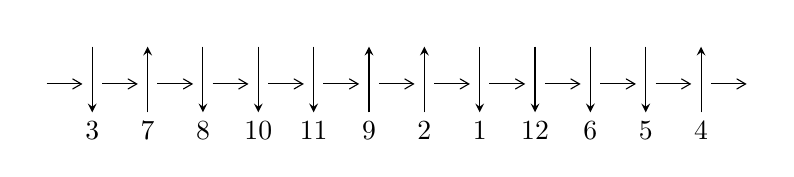
\begin{tikzpicture}[x=20pt, y=17pt]
	% nodes
	\node (C0) at (0, 0) {};
	\node (C1) at (1, 0) {};
	\node (C1U) at (1, +1) {};
	\node (C1D) at (1, -1) {3};

	\node (C2) at (2, 0) {};
	\node (C2U) at (2, +1) {};
	\node (C2D) at (2, -1) {7};

	\node (C3) at (3, 0) {};
	\node (C3U) at (3, +1) {};
	\node (C3D) at (3, -1) {8};

	\node (C4) at (4, 0) {};
	\node (C4U) at (4, +1) {};
	\node (C4D) at (4, -1) {10};

	\node (C5) at (5, 0) {};
	\node (C5U) at (5, +1) {};
	\node (C5D) at (5, -1) {11};

	\node (C6) at (6, 0) {};
	\node (C6U) at (6, +1) {};
	\node (C6D) at (6, -1) {9};

	\node (C7) at (7, 0) {};
	\node (C7U) at (7, +1) {};
	\node (C7D) at (7, -1) {2};

	\node (C8) at (8, 0) {};
	\node (C8U) at (8, +1) {};
	\node (C8D) at (8, -1) {1};

	\node (C9) at (9, 0) {};
	\node (C9U) at (9, +1) {};
	\node (C9D) at (9, -1) {12};

	\node (C10) at (10, 0) {};
	\node (C10U) at (10, +1) {};
	\node (C10D) at (10, -1) {6};

	\node (C11) at (11, 0) {};
	\node (C11U) at (11, +1) {};
	\node (C11D) at (11, -1) {5};

	\node (C12) at (12, 0) {};
	\node (C12U) at (12, +1) {};
	\node (C12D) at (12, -1) {4};
	\node (C13) at (13, 0) {};

	% arrows
	\draw[->,>={angle 60}]
	(C0) edge (C1) (C1) edge (C2) (C2) edge (C3) (C3) edge (C4) (C4) edge (C5) (C5) edge (C6) (C6) edge (C7) (C7) edge (C8) (C8) edge (C9) (C9) edge (C10) (C10) edge (C11) (C11) edge (C12) (C12) edge (C13) ;	\draw[->,>=stealth]
	(C1U) edge (C1D) (C2D) edge (C2U) (C3U) edge (C3D) (C4U) edge (C4D) (C5U) edge (C5D) (C6D) edge (C6U) (C7D) edge (C7U) (C8U) edge (C8D) (C9U) edge (C9D) (C10U) edge (C10D) (C11U) edge (C11D) (C12D) edge (C12U) ;
	\end{tikzpicture} \\
\hhline{~~} \\& 
\textbf{Solving Sequence} \\ \cline{2-2} 
 &
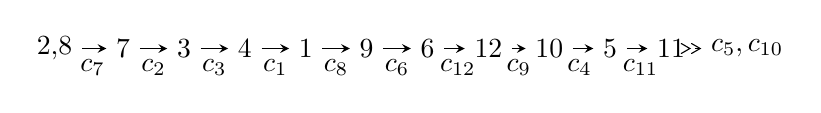
\begin{tikzpicture}[x=22pt, y=7pt]
	% node
	\node (A0) at (-1/8, 0) {2,8};
	\node (A1) at (1, 0) {7};
	\node (A2) at (2, 0) {3};
	\node (A3) at (3, 0) {4};
	\node (A4) at (4, 0) {1};
	\node (A5) at (5, 0) {9};
	\node (A6) at (6, 0) {6};
	\node (A7) at (7, 0) {12};
	\node (A8) at (8, 0) {10};
	\node (A9) at (9, 0) {5};
	\node (A10) at (10, 0) {11};
	\node (C1) at (1/2, -1) {$c_{7}$};
	\node (C2) at (3/2, -1) {$c_{2}$};
	\node (C3) at (5/2, -1) {$c_{3}$};
	\node (C4) at (7/2, -1) {$c_{1}$};
	\node (C5) at (9/2, -1) {$c_{8}$};
	\node (C6) at (11/2, -1) {$c_{6}$};
	\node (C7) at (13/2, -1) {$c_{12}$};
	\node (C8) at (15/2, -1) {$c_{9}$};
	\node (C9) at (17/2, -1) {$c_{4}$};
	\node (C10) at (19/2, -1) {$c_{11}$};
	\node (A11) at (45/4, 0) {$c_{5},c_{10}$};

	% edge
	\draw[->,>=stealth]	
	(A0) edge (A1) (A1) edge (A2) (A2) edge (A3) (A3) edge (A4) (A4) edge (A5) (A5) edge (A6) (A6) edge (A7) (A7) edge (A8) (A8) edge (A9) (A9) edge (A10) ;
	\draw[->>,>={angle 60}]	
	(A10) edge (A11);
\end{tikzpicture} \\ 

\end{tabular} \\

\footnotetext{
The image of knot diagram is generated by the software ``\textbf{Draw programme}" developed by Andrew Bartholomew(\url{http://www.layer8.co.uk/maths/draw/index.htm\#Running-draw}), where we modified some parts for our purpose(\url{https://github.com/CATsTAILs/LinksPainter}).
}\phantom \\ \newline 
\centering \textbf{Ideals for irreducible components\footnotemark of $X_{\text{par}}$} 
 
\begin{align*}
I^u_{1}&=\langle 
u^{89}- u^{88}+\cdots+u-1\rangle \\
\\
\end{align*}
\raggedright * 1 irreducible components of $\dim_{\mathbb{C}}=0$, with total 89 representations.\\
\footnotetext{All coefficients of polynomials are rational numbers. But the coefficients are sometimes approximated in decimal forms when there is not enough margin.}
\newpage
\renewcommand{\arraystretch}{1}
\centering \section*{I. $I^u_{1}= \langle u^{89}- u^{88}+\cdots+u-1 \rangle$}
\flushleft \textbf{(i) Arc colorings}\\
\begin{tabular}{m{7pt} m{180pt} m{7pt} m{180pt} }
\flushright $a_{2}=$&$\begin{pmatrix}0\\u\end{pmatrix}$ \\
\flushright $a_{8}=$&$\begin{pmatrix}1\\0\end{pmatrix}$ \\
\flushright $a_{7}=$&$\begin{pmatrix}1\\u^2\end{pmatrix}$ \\
\flushright $a_{3}=$&$\begin{pmatrix}u\\u^3+u\end{pmatrix}$ \\
\flushright $a_{4}=$&$\begin{pmatrix}- u^3\\u^3+u\end{pmatrix}$ \\
\flushright $a_{1}=$&$\begin{pmatrix}u^3\\u^5+u^3+u\end{pmatrix}$ \\
\flushright $a_{9}=$&$\begin{pmatrix}u^8+u^6+u^4+1\\u^{10}+2 u^8+3 u^6+2 u^4+u^2\end{pmatrix}$ \\
\flushright $a_{6}=$&$\begin{pmatrix}u^{16}+3 u^{14}+5 u^{12}+4 u^{10}+3 u^8+2 u^6+2 u^4+1\\u^{18}+4 u^{16}+9 u^{14}+12 u^{12}+11 u^{10}+6 u^8+2 u^6+u^2\end{pmatrix}$ \\
\flushright $a_{12}=$&$\begin{pmatrix}- u^{11}-2 u^9-2 u^7+u^3\\u^{11}+3 u^9+4 u^7+3 u^5+u^3+u\end{pmatrix}$ \\
\flushright $a_{10}=$&$\begin{pmatrix}- u^{32}-7 u^{30}+\cdots+2 u^4+1\\u^{32}+8 u^{30}+\cdots+4 u^4+2 u^2\end{pmatrix}$ \\
\flushright $a_{5}=$&$\begin{pmatrix}u^{61}+14 u^{59}+\cdots-2 u^3- u\\- u^{61}-15 u^{59}+\cdots- u^3+u\end{pmatrix}$ \\
\flushright $a_{11}=$&$\begin{pmatrix}- u^{66}-15 u^{64}+\cdots- u^2+1\\- u^{68}-16 u^{66}+\cdots+3 u^4+2 u^2\end{pmatrix}$\\&\end{tabular}
\flushleft \textbf{(ii) Obstruction class $= -1$}\\~\\
\flushleft \textbf{(iii) Cusp Shapes $= 4 u^{87}-4 u^{86}+\cdots-4 u^2-6$}\\~\\
\newpage\renewcommand{\arraystretch}{1}
\flushleft \textbf{(iv) u-Polynomials at the component}\newline \\
\begin{tabular}{m{50pt}|m{274pt}}
Crossings & \hspace{64pt}u-Polynomials at each crossing \\
\hline $$\begin{aligned}c_{1}\end{aligned}$$&$\begin{aligned}
&u^{89}+43 u^{88}+\cdots+u-1
\end{aligned}$\\
\hline $$\begin{aligned}c_{2},c_{7}\end{aligned}$$&$\begin{aligned}
&u^{89}+u^{88}+\cdots+u+1
\end{aligned}$\\
\hline $$\begin{aligned}c_{3}\end{aligned}$$&$\begin{aligned}
&u^{89}- u^{88}+\cdots+1497 u+457
\end{aligned}$\\
\hline $$\begin{aligned}c_{4}\end{aligned}$$&$\begin{aligned}
&u^{89}- u^{88}+\cdots-5 u+1
\end{aligned}$\\
\hline $$\begin{aligned}c_{5},c_{10},c_{11}\end{aligned}$$&$\begin{aligned}
&u^{89}+u^{88}+\cdots+3 u+1
\end{aligned}$\\
\hline $$\begin{aligned}c_{6},c_{12}\end{aligned}$$&$\begin{aligned}
&u^{89}+7 u^{88}+\cdots+161 u+5
\end{aligned}$\\
\hline $$\begin{aligned}c_{8}\end{aligned}$$&$\begin{aligned}
&u^{89}+5 u^{88}+\cdots+u+1
\end{aligned}$\\
\hline $$\begin{aligned}c_{9}\end{aligned}$$&$\begin{aligned}
&u^{89}-21 u^{88}+\cdots-4023 u+187
\end{aligned}$\\
\hline
\end{tabular}\\~\\
\newpage\renewcommand{\arraystretch}{1}
\flushleft \textbf{(v) Riley Polynomials at the component}\newline \\
\begin{tabular}{m{50pt}|m{274pt}}
Crossings & \hspace{64pt}Riley Polynomials at each crossing \\
\hline $$\begin{aligned}c_{1}\end{aligned}$$&$\begin{aligned}
&y^{89}+7 y^{88}+\cdots+13 y-1
\end{aligned}$\\
\hline $$\begin{aligned}c_{2},c_{7}\end{aligned}$$&$\begin{aligned}
&y^{89}+43 y^{88}+\cdots+y-1
\end{aligned}$\\
\hline $$\begin{aligned}c_{3}\end{aligned}$$&$\begin{aligned}
&y^{89}-29 y^{88}+\cdots+6081637 y-208849
\end{aligned}$\\
\hline $$\begin{aligned}c_{4}\end{aligned}$$&$\begin{aligned}
&y^{89}-5 y^{88}+\cdots+17 y-1
\end{aligned}$\\
\hline $$\begin{aligned}c_{5},c_{10},c_{11}\end{aligned}$$&$\begin{aligned}
&y^{89}+79 y^{88}+\cdots+y-1
\end{aligned}$\\
\hline $$\begin{aligned}c_{6},c_{12}\end{aligned}$$&$\begin{aligned}
&y^{89}+67 y^{88}+\cdots+201 y-25
\end{aligned}$\\
\hline $$\begin{aligned}c_{8}\end{aligned}$$&$\begin{aligned}
&y^{89}- y^{88}+\cdots+61 y-1
\end{aligned}$\\
\hline $$\begin{aligned}c_{9}\end{aligned}$$&$\begin{aligned}
&y^{89}+11 y^{88}+\cdots-1504923 y-34969
\end{aligned}$\\
\hline
\end{tabular}\\~\\
\newpage\flushleft \textbf{(vi) Complex Volumes and Cusp Shapes}
$$\begin{array}{c|c|c}  
\text{Solutions to }I^u_{1}& \I (\text{vol} + \sqrt{-1}CS) & \text{Cusp shape}\\
 \hline 
\begin{aligned}
u &= -0.549845 + 0.852652 I\end{aligned}
 & \phantom{-}3.32155 + 4.57387 I & \phantom{-0.000000 } 0 \\ \hline\begin{aligned}
u &= -0.549845 - 0.852652 I\end{aligned}
 & \phantom{-}3.32155 - 4.57387 I & \phantom{-0.000000 } 0 \\ \hline\begin{aligned}
u &= \phantom{-}0.526296 + 0.826367 I\end{aligned}
 & -1.86086 - 1.10863 I & \phantom{-0.000000 } 0 \\ \hline\begin{aligned}
u &= \phantom{-}0.526296 - 0.826367 I\end{aligned}
 & -1.86086 + 1.10863 I & \phantom{-0.000000 } 0 \\ \hline\begin{aligned}
u &= -0.445113 + 0.947902 I\end{aligned}
 & -0.40489 - 1.97636 I & \phantom{-0.000000 } 0 \\ \hline\begin{aligned}
u &= -0.445113 - 0.947902 I\end{aligned}
 & -0.40489 + 1.97636 I & \phantom{-0.000000 } 0 \\ \hline\begin{aligned}
u &= -0.130520 + 0.933837 I\end{aligned}
 & \phantom{-}3.46999 + 3.77804 I & -4.00000 - 3.55964 I \\ \hline\begin{aligned}
u &= -0.130520 - 0.933837 I\end{aligned}
 & \phantom{-}3.46999 - 3.77804 I & -4.00000 + 3.55964 I \\ \hline\begin{aligned}
u &= \phantom{-}0.237242 + 0.899093 I\end{aligned}
 & -1.63382 - 0.87283 I & -8.59634 + 3.63079 I \\ \hline\begin{aligned}
u &= \phantom{-}0.237242 - 0.899093 I\end{aligned}
 & -1.63382 + 0.87283 I & -8.59634 - 3.63079 I \\ \hline\begin{aligned}
u &= -0.621956 + 0.688948 I\end{aligned}
 & \phantom{-}3.81774 - 9.21070 I & \phantom{-0.000000 -}0. + 8.07606 I \\ \hline\begin{aligned}
u &= -0.621956 - 0.688948 I\end{aligned}
 & \phantom{-}3.81774 + 9.21070 I & \phantom{-0.000000 } 0. - 8.07606 I \\ \hline\begin{aligned}
u &= \phantom{-}0.605630 + 0.694228 I\end{aligned}
 & -1.43820 + 5.63420 I & -4.00000 - 7.71170 I \\ \hline\begin{aligned}
u &= \phantom{-}0.605630 - 0.694228 I\end{aligned}
 & -1.43820 - 5.63420 I & -4.00000 + 7.71170 I \\ \hline\begin{aligned}
u &= \phantom{-}0.523965 + 0.945138 I\end{aligned}
 & \phantom{-}5.28882 + 3.53448 I & \phantom{-0.000000 } 0 \\ \hline\begin{aligned}
u &= \phantom{-}0.523965 - 0.945138 I\end{aligned}
 & \phantom{-}5.28882 - 3.53448 I & \phantom{-0.000000 } 0 \\ \hline\begin{aligned}
u &= -0.544235 + 0.732626 I\end{aligned}
 & \phantom{-}0.19552 - 2.15749 I & -2.95032 + 4.14794 I \\ \hline\begin{aligned}
u &= -0.544235 - 0.732626 I\end{aligned}
 & \phantom{-}0.19552 + 2.15749 I & -2.95032 - 4.14794 I \\ \hline\begin{aligned}
u &= -0.556700 + 0.687523 I\end{aligned}
 & \phantom{-}0.25637 - 2.05649 I & -1.44246 + 3.13624 I \\ \hline\begin{aligned}
u &= -0.556700 - 0.687523 I\end{aligned}
 & \phantom{-}0.25637 + 2.05649 I & -1.44246 - 3.13624 I \\ \hline\begin{aligned}
u &= \phantom{-}0.601306 + 0.620005 I\end{aligned}
 & \phantom{-}6.23656 + 0.95324 I & \phantom{-}3.59693 - 2.99187 I \\ \hline\begin{aligned}
u &= \phantom{-}0.601306 - 0.620005 I\end{aligned}
 & \phantom{-}6.23656 - 0.95324 I & \phantom{-}3.59693 + 2.99187 I \\ \hline\begin{aligned}
u &= -0.389004 + 1.075220 I\end{aligned}
 & -0.038564 - 0.742399 I & \phantom{-0.000000 } 0 \\ \hline\begin{aligned}
u &= -0.389004 - 1.075220 I\end{aligned}
 & -0.038564 + 0.742399 I & \phantom{-0.000000 } 0 \\ \hline\begin{aligned}
u &= -0.270428 + 1.114400 I\end{aligned}
 & \phantom{-}0.573665 - 0.094345 I & \phantom{-0.000000 } 0 \\ \hline\begin{aligned}
u &= -0.270428 - 1.114400 I\end{aligned}
 & \phantom{-}0.573665 + 0.094345 I & \phantom{-0.000000 } 0 \\ \hline\begin{aligned}
u &= \phantom{-}0.443236 + 1.076980 I\end{aligned}
 & -3.58294 + 3.54004 I & \phantom{-0.000000 } 0 \\ \hline\begin{aligned}
u &= \phantom{-}0.443236 - 1.076980 I\end{aligned}
 & -3.58294 - 3.54004 I & \phantom{-0.000000 } 0 \\ \hline\begin{aligned}
u &= \phantom{-}0.773116 + 0.297168 I\end{aligned}
 & \phantom{-}1.90632 - 11.11310 I & -1.08984 + 6.87770 I \\ \hline\begin{aligned}
u &= \phantom{-}0.773116 - 0.297168 I\end{aligned}
 & \phantom{-}1.90632 + 11.11310 I & -1.08984 - 6.87770 I\\
 \hline 
 \end{array}$$\newpage$$\begin{array}{c|c|c}  
\text{Solutions to }I^u_{1}& \I (\text{vol} + \sqrt{-1}CS) & \text{Cusp shape}\\
 \hline 
\begin{aligned}
u &= \phantom{-}0.555744 + 1.035790 I\end{aligned}
 & \phantom{-}6.42783 + 1.42029 I & \phantom{-0.000000 } 0 \\ \hline\begin{aligned}
u &= \phantom{-}0.555744 - 1.035790 I\end{aligned}
 & \phantom{-}6.42783 - 1.42029 I & \phantom{-0.000000 } 0 \\ \hline\begin{aligned}
u &= -0.537606 + 1.047480 I\end{aligned}
 & \phantom{-}0.71771 - 3.82158 I & \phantom{-0.000000 } 0 \\ \hline\begin{aligned}
u &= -0.537606 - 1.047480 I\end{aligned}
 & \phantom{-}0.71771 + 3.82158 I & \phantom{-0.000000 } 0 \\ \hline\begin{aligned}
u &= -0.767527 + 0.290372 I\end{aligned}
 & -3.36844 + 7.41224 I & -5.77885 - 6.28864 I \\ \hline\begin{aligned}
u &= -0.767527 - 0.290372 I\end{aligned}
 & -3.36844 - 7.41224 I & -5.77885 + 6.28864 I \\ \hline\begin{aligned}
u &= \phantom{-}0.654390 + 0.489201 I\end{aligned}
 & \phantom{-}8.03046 + 3.30236 I & \phantom{-}5.19136 - 3.35930 I \\ \hline\begin{aligned}
u &= \phantom{-}0.654390 - 0.489201 I\end{aligned}
 & \phantom{-}8.03046 - 3.30236 I & \phantom{-}5.19136 + 3.35930 I \\ \hline\begin{aligned}
u &= \phantom{-}0.280299 + 1.149490 I\end{aligned}
 & -5.92026 - 0.49034 I & \phantom{-0.000000 } 0 \\ \hline\begin{aligned}
u &= \phantom{-}0.280299 - 1.149490 I\end{aligned}
 & -5.92026 + 0.49034 I & \phantom{-0.000000 } 0 \\ \hline\begin{aligned}
u &= \phantom{-}0.260330 + 1.156600 I\end{aligned}
 & -2.58902 - 8.08324 I & \phantom{-0.000000 } 0 \\ \hline\begin{aligned}
u &= \phantom{-}0.260330 - 1.156600 I\end{aligned}
 & -2.58902 + 8.08324 I & \phantom{-0.000000 } 0 \\ \hline\begin{aligned}
u &= -0.267783 + 1.155220 I\end{aligned}
 & -7.80687 + 4.35790 I & \phantom{-0.000000 } 0 \\ \hline\begin{aligned}
u &= -0.267783 - 1.155220 I\end{aligned}
 & -7.80687 - 4.35790 I & \phantom{-0.000000 } 0 \\ \hline\begin{aligned}
u &= \phantom{-}0.293939 + 1.151340 I\end{aligned}
 & -6.07434 - 0.28887 I & \phantom{-0.000000 } 0 \\ \hline\begin{aligned}
u &= \phantom{-}0.293939 - 1.151340 I\end{aligned}
 & -6.07434 + 0.28887 I & \phantom{-0.000000 } 0 \\ \hline\begin{aligned}
u &= -0.683893 + 0.428051 I\end{aligned}
 & \phantom{-}7.74822 + 5.29418 I & \phantom{-}4.36161 - 4.33354 I \\ \hline\begin{aligned}
u &= -0.683893 - 0.428051 I\end{aligned}
 & \phantom{-}7.74822 - 5.29418 I & \phantom{-}4.36161 + 4.33354 I \\ \hline\begin{aligned}
u &= -0.308826 + 1.154160 I\end{aligned}
 & -8.28930 - 3.48798 I & \phantom{-0.000000 } 0 \\ \hline\begin{aligned}
u &= -0.308826 - 1.154160 I\end{aligned}
 & -8.28930 + 3.48798 I & \phantom{-0.000000 } 0 \\ \hline\begin{aligned}
u &= -0.471075 + 1.098060 I\end{aligned}
 & \phantom{-}0.51569 - 6.51976 I & \phantom{-0.000000 } 0 \\ \hline\begin{aligned}
u &= -0.471075 - 1.098060 I\end{aligned}
 & \phantom{-}0.51569 + 6.51976 I & \phantom{-0.000000 } 0 \\ \hline\begin{aligned}
u &= \phantom{-}0.752387 + 0.281402 I\end{aligned}
 & -1.59860 - 3.55841 I & -3.12371 + 1.57420 I \\ \hline\begin{aligned}
u &= \phantom{-}0.752387 - 0.281402 I\end{aligned}
 & -1.59860 + 3.55841 I & -3.12371 - 1.57420 I \\ \hline\begin{aligned}
u &= \phantom{-}0.318069 + 1.155530 I\end{aligned}
 & -3.26936 + 7.19305 I & \phantom{-0.000000 } 0 \\ \hline\begin{aligned}
u &= \phantom{-}0.318069 - 1.155530 I\end{aligned}
 & -3.26936 - 7.19305 I & \phantom{-0.000000 } 0 \\ \hline\begin{aligned}
u &= -0.734105 + 0.315100 I\end{aligned}
 & \phantom{-}4.84491 + 2.69309 I & \phantom{-}1.74893 - 2.46850 I \\ \hline\begin{aligned}
u &= -0.734105 - 0.315100 I\end{aligned}
 & \phantom{-}4.84491 - 2.69309 I & \phantom{-}1.74893 + 2.46850 I \\ \hline\begin{aligned}
u &= \phantom{-}0.548293 + 1.068850 I\end{aligned}
 & \phantom{-}0.30757 + 7.15974 I & \phantom{-0.000000 } 0 \\ \hline\begin{aligned}
u &= \phantom{-}0.548293 - 1.068850 I\end{aligned}
 & \phantom{-}0.30757 - 7.15974 I & \phantom{-0.000000 } 0\\
 \hline 
 \end{array}$$\newpage$$\begin{array}{c|c|c}  
\text{Solutions to }I^u_{1}& \I (\text{vol} + \sqrt{-1}CS) & \text{Cusp shape}\\
 \hline 
\begin{aligned}
u &= -0.561612 + 1.069280 I\end{aligned}
 & \phantom{-}5.87439 - 10.10820 I & \phantom{-0.000000 } 0 \\ \hline\begin{aligned}
u &= -0.561612 - 1.069280 I\end{aligned}
 & \phantom{-}5.87439 + 10.10820 I & \phantom{-0.000000 } 0 \\ \hline\begin{aligned}
u &= \phantom{-}0.746796 + 0.262051 I\end{aligned}
 & -1.84029 - 3.44425 I & -4.01435 + 3.41599 I \\ \hline\begin{aligned}
u &= \phantom{-}0.746796 - 0.262051 I\end{aligned}
 & -1.84029 + 3.44425 I & -4.01435 - 3.41599 I \\ \hline\begin{aligned}
u &= -0.621550 + 0.465042 I\end{aligned}
 & \phantom{-}2.42382 - 0.75571 I & \phantom{-}1.71757 + 3.84156 I \\ \hline\begin{aligned}
u &= -0.621550 - 0.465042 I\end{aligned}
 & \phantom{-}2.42382 + 0.75571 I & \phantom{-}1.71757 - 3.84156 I \\ \hline\begin{aligned}
u &= \phantom{-}0.653966 + 0.417174 I\end{aligned}
 & \phantom{-}2.20293 - 2.46586 I & \phantom{-}0.44156 + 5.21162 I \\ \hline\begin{aligned}
u &= \phantom{-}0.653966 - 0.417174 I\end{aligned}
 & \phantom{-}2.20293 + 2.46586 I & \phantom{-}0.44156 - 5.21162 I \\ \hline\begin{aligned}
u &= -0.737893 + 0.238500 I\end{aligned}
 & -4.15809 - 0.23287 I & -7.53192 + 1.38224 I \\ \hline\begin{aligned}
u &= -0.737893 - 0.238500 I\end{aligned}
 & -4.15809 + 0.23287 I & -7.53192 - 1.38224 I \\ \hline\begin{aligned}
u &= \phantom{-}0.733536 + 0.221566 I\end{aligned}
 & \phantom{-}0.79810 + 3.87164 I & -2.73189 - 2.63327 I \\ \hline\begin{aligned}
u &= \phantom{-}0.733536 - 0.221566 I\end{aligned}
 & \phantom{-}0.79810 - 3.87164 I & -2.73189 + 2.63327 I \\ \hline\begin{aligned}
u &= -0.553875 + 1.124130 I\end{aligned}
 & \phantom{-}2.48561 - 7.58332 I & \phantom{-0.000000 } 0 \\ \hline\begin{aligned}
u &= -0.553875 - 1.124130 I\end{aligned}
 & \phantom{-}2.48561 + 7.58332 I & \phantom{-0.000000 } 0 \\ \hline\begin{aligned}
u &= \phantom{-}0.526277 + 1.142710 I\end{aligned}
 & -1.85636 + 0.86225 I & \phantom{-0.000000 } 0 \\ \hline\begin{aligned}
u &= \phantom{-}0.526277 - 1.142710 I\end{aligned}
 & -1.85636 - 0.86225 I & \phantom{-0.000000 } 0 \\ \hline\begin{aligned}
u &= -0.532862 + 1.141630 I\end{aligned}
 & -6.76881 - 4.54935 I & \phantom{-0.000000 } 0 \\ \hline\begin{aligned}
u &= -0.532862 - 1.141630 I\end{aligned}
 & -6.76881 + 4.54935 I & \phantom{-0.000000 } 0 \\ \hline\begin{aligned}
u &= \phantom{-}0.541979 + 1.140190 I\end{aligned}
 & -4.39315 + 8.29738 I & \phantom{-0.000000 } 0 \\ \hline\begin{aligned}
u &= \phantom{-}0.541979 - 1.140190 I\end{aligned}
 & -4.39315 - 8.29738 I & \phantom{-0.000000 } 0 \\ \hline\begin{aligned}
u &= \phantom{-}0.549916 + 1.137700 I\end{aligned}
 & -4.09560 + 8.46534 I & \phantom{-0.000000 } 0 \\ \hline\begin{aligned}
u &= \phantom{-}0.549916 - 1.137700 I\end{aligned}
 & -4.09560 - 8.46534 I & \phantom{-0.000000 } 0 \\ \hline\begin{aligned}
u &= -0.556243 + 1.140170 I\end{aligned}
 & -5.85930 - 12.38420 I & \phantom{-0.000000 } 0 \\ \hline\begin{aligned}
u &= -0.556243 - 1.140170 I\end{aligned}
 & -5.85930 + 12.38420 I & \phantom{-0.000000 } 0 \\ \hline\begin{aligned}
u &= \phantom{-}0.559891 + 1.140150 I\end{aligned}
 & -0.5695 + 16.1155 I & \phantom{-0.000000 } 0 \\ \hline\begin{aligned}
u &= \phantom{-}0.559891 - 1.140150 I\end{aligned}
 & -0.5695 - 16.1155 I & \phantom{-0.000000 } 0 \\ \hline\begin{aligned}
u &= -0.570709 + 0.131663 I\end{aligned}
 & \phantom{-}3.08005 + 2.48479 I & -2.33160 - 3.10830 I \\ \hline\begin{aligned}
u &= -0.570709 - 0.131663 I\end{aligned}
 & \phantom{-}3.08005 - 2.48479 I & -2.33160 + 3.10830 I \\ \hline\begin{aligned}
u &= \phantom{-}0.453510\phantom{ +0.000000I}\end{aligned}
 & -1.01886\phantom{ +0.000000I} & -9.58030\phantom{ +0.000000I}\\
 \hline 
 \end{array}$$\newpage
\newpage\renewcommand{\arraystretch}{1}
\centering \section*{ II. u-Polynomials}
\begin{tabular}{m{50pt}|m{274pt}}
Crossings & \hspace{64pt}u-Polynomials at each crossing \\
\hline $$\begin{aligned}c_{1}\end{aligned}$$&$\begin{aligned}
&u^{89}+43 u^{88}+\cdots+u-1
\end{aligned}$\\
\hline $$\begin{aligned}c_{2},c_{7}\end{aligned}$$&$\begin{aligned}
&u^{89}+u^{88}+\cdots+u+1
\end{aligned}$\\
\hline $$\begin{aligned}c_{3}\end{aligned}$$&$\begin{aligned}
&u^{89}- u^{88}+\cdots+1497 u+457
\end{aligned}$\\
\hline $$\begin{aligned}c_{4}\end{aligned}$$&$\begin{aligned}
&u^{89}- u^{88}+\cdots-5 u+1
\end{aligned}$\\
\hline $$\begin{aligned}c_{5},c_{10},c_{11}\end{aligned}$$&$\begin{aligned}
&u^{89}+u^{88}+\cdots+3 u+1
\end{aligned}$\\
\hline $$\begin{aligned}c_{6},c_{12}\end{aligned}$$&$\begin{aligned}
&u^{89}+7 u^{88}+\cdots+161 u+5
\end{aligned}$\\
\hline $$\begin{aligned}c_{8}\end{aligned}$$&$\begin{aligned}
&u^{89}+5 u^{88}+\cdots+u+1
\end{aligned}$\\
\hline $$\begin{aligned}c_{9}\end{aligned}$$&$\begin{aligned}
&u^{89}-21 u^{88}+\cdots-4023 u+187
\end{aligned}$\\
\hline
\end{tabular}\newpage\renewcommand{\arraystretch}{1}
\centering \section*{ III. Riley Polynomials}
\begin{tabular}{m{50pt}|m{274pt}}
Crossings & \hspace{64pt}Riley Polynomials at each crossing \\
\hline $$\begin{aligned}c_{1}\end{aligned}$$&$\begin{aligned}
&y^{89}+7 y^{88}+\cdots+13 y-1
\end{aligned}$\\
\hline $$\begin{aligned}c_{2},c_{7}\end{aligned}$$&$\begin{aligned}
&y^{89}+43 y^{88}+\cdots+y-1
\end{aligned}$\\
\hline $$\begin{aligned}c_{3}\end{aligned}$$&$\begin{aligned}
&y^{89}-29 y^{88}+\cdots+6081637 y-208849
\end{aligned}$\\
\hline $$\begin{aligned}c_{4}\end{aligned}$$&$\begin{aligned}
&y^{89}-5 y^{88}+\cdots+17 y-1
\end{aligned}$\\
\hline $$\begin{aligned}c_{5},c_{10},c_{11}\end{aligned}$$&$\begin{aligned}
&y^{89}+79 y^{88}+\cdots+y-1
\end{aligned}$\\
\hline $$\begin{aligned}c_{6},c_{12}\end{aligned}$$&$\begin{aligned}
&y^{89}+67 y^{88}+\cdots+201 y-25
\end{aligned}$\\
\hline $$\begin{aligned}c_{8}\end{aligned}$$&$\begin{aligned}
&y^{89}- y^{88}+\cdots+61 y-1
\end{aligned}$\\
\hline $$\begin{aligned}c_{9}\end{aligned}$$&$\begin{aligned}
&y^{89}+11 y^{88}+\cdots-1504923 y-34969
\end{aligned}$\\
\hline
\end{tabular}
\vskip 2pc
\end{document}